\documentclass{article}

\usepackage{graphicx}

\begin{document}
	\section*{Lab3 - Filip Jędrzejewski}
	
	\subsection*{Opis problemu}
	
	Populacja Stanów Zjednoczonych na przestrzeni lat przedstawiała się następujaco:
	
	\begin{center}
		\begin{tabular}{c|c}
  			\hline 
  			Rok & Populacja\\
  			\hline
  			1900 & 76 212 168 \\
  			1910 & 92 228 496 \\
  			1920 & 106 021 537 \\
  			1930 & 123 202 624 \\
  			1940 & 132 164 569 \\
  			1950 & 151 325 798 \\
  			1960 & 179 323 175 \\
  			1970 & 203 302 031 \\
  			1980 & 226 542 199 \\
		\end{tabular} 
		
	\end{center}
	
	W celu wyznaczenia wielomianu, który interpoluje powyższe dziewięć punktów rozważono następujące zbiory funkcji bazowych $\phi (t)$, $j=1,2,...,9$:
	
	\begin{equation}
		\phi_j (t) = t^{j-1}
	\end{equation}
	
	\begin{equation}
		\phi_j (t) = (t-1900)^{j-1}
	\end{equation}
	
	\begin{equation}
		\phi_j (t) = (t-1940)^{j-1}
	\end{equation}
	
	\begin{equation}
		\phi_j (t) = \left(\frac{t-1940}{40}\right)^{j-1}
	\end{equation}
	
	\subsection*{Wyznaczanie wielomianu za pomocą macierzy}
	
	Dla każdego z czterech zbiorów funkcji bazowych utworzono macierz Vandermonde'a, a następnie korzystając z funkcji \texttt{numpy.linalg.cond} obliczono współczynniki uwarunkowania każdej z nich. Wyniki przedstawiono w tabeli: 
	
	\begin{center}
		\begin{tabular}{|c|c|}
  			\hline 
  			Numer funkcji bazowej & Współczynnik uwarunkowania macierzy\\
  			\hline
  			1 & $5.031 \cdot 10^{26}$ \\
  			2 & $6.307 \cdot 10^{15}$ \\
  			3 & $9.316 \cdot 10^{12}$ \\
  			4 & $1.605 \cdot 10^{3}$ \\
  			\hline
		\end{tabular} 
		
	\end{center}
	
	Najmniejszy współczynnik uwarunkowania miała baza określona wzorem (4), zatem została ona wybrana do wynaczenia wielomianu interpolacyjnego. W tym celu rozwiązano następujące równanie macierzowe:
	
	\begin{equation}
		M \cdot C = Y
	\end{equation}
	
	przy czym: $M$ - macierz Vandermonde'a utworzona na najlepiej uwarunkowanej bazie, $C$ - szukana macierz współczynników, $Y$ - macierz wartości wielomianu dla danych punktów (pierwsza tabela). \\
	Do rozwiązania tego równania użyto funkcji \texttt{numpy.linalg.solve}, która zwraca rozwiązanie równania macierzowego typu $AX=B$, gdzie $A$ i $B$ są dane, a $X$ szukana. \\
	W kolejnym kroku utworzono wykres otrzymanego wielomianu na przedziale $year \in [1900, 1990]$, na który naniesiono węzły interpolacji.
	
	
	\begin{figure}[h]
    		\centering
  		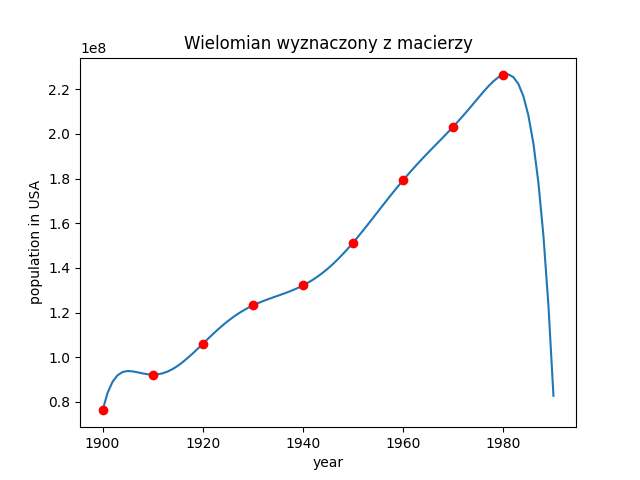
\includegraphics[scale = 0.9]{wykres1.png}
	\end{figure}
	
	Wykres wielomianu interpolacyjnego przechodzi przez wszystkie dziewięć węzłow interpolacji, co potwierdza poprawność wykonanej interpolacji.\\
	Kolejną czynnością było dokonanie ekstrapolacji wielomianu do 1990 roku. Otrzymano wartość $82749141$, która w porównaniu prawdziwej wartości populacji dla Stanów Zjednoczonych w 1990 roku, równej $248709873$, miała błąd względny ekstrapolacji równy:
	
	\begin{equation}
		relativeExtrapolationError = 0.6672864651416437 \approx 66.73 \%
	\end{equation}
	
	
	
	\subsection*{Wyznaczanie wielomianu Lagrange'a}
	
	W celu wyznaczenia wielomianu interpolacyjnego Lagrange'a użyto następujacych wzorów:
	
	\begin{equation}
		l_j (t) = \prod _{k=1, k \neq j} ^ n \frac{t-t_k}{t_j - t_k}
	\end{equation}
	
	\begin{equation}
		p (t) = \sum _{i=1} ^n y_i  l_i(t)
	\end{equation}
	
	Na ich podstawie, korzystajac z funkcji \texttt{lambda}, wyznaczono wielomian interpolacyjny Lagrange'a. Nastepnie obliczono wartości tego wielomianu dla takiego samego przedziału jak w poprzednim podpunkcie z krokiem co jeden rok. Na podstawie uzyskanych wartości stworzono wykres:
	
	\begin{figure}[h]
    		\centering
  		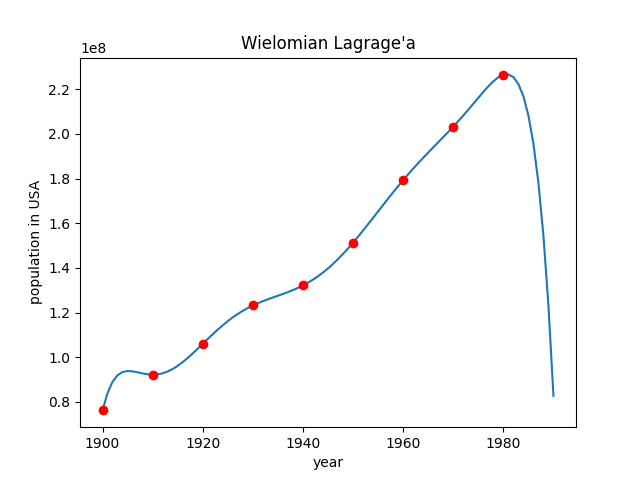
\includegraphics[scale = 0.9]{wykres2.png}
	\end{figure}
	
	Powyższy wykres jest identyczny jak ten stworzony na podstawie macierzy, co potwierdza poprawność wyznaczenia wielomianu metodą Lagrange'a.
	
	
	\subsection*{Wyznaczanie wielomianu Newtona}
	
	W celu wyznaczenia wielomianu interpolacyjnego Newtona użyto następujących wzorów:
	
	\begin{equation}
		\pi (t) = \prod _{k=1} ^ {j-1} (t-t_k)
	\end{equation}
	
	\begin{equation}
		p (t) = \sum _{i=1} ^n f[t_1,...,t_i] \cdot \pi_i(t)
	\end{equation}
	
	\begin{equation}
		f[x_i] = f(x_i)
	\end{equation}
	
	\begin{equation}
		f[x_i, x_{i+1}] = \frac{f[x_{i+1}]-f[x_{i}]}{x_{i+1} - x_{i}}
	\end{equation}
	
	\begin{equation}
		f[x_0, ..., x_i] = \frac{f[x_1, ..., x_i] - f[x_0,...,x_{i-1}]}{x_i - x_0}
	\end{equation}
	
	Na ich podstawie, korzystajac z funkcji \texttt{lambda} oraz rekurencyjnie obliczając wartości ilorazów różnicowych, wyznaczono wielomian interpolacyjny Newtona. Następnie obliczono wartości tego wielomianu dla takiego samego przedziału jak w pierwszym podpunkcie z krokiem co jeden rok. Na podstawie uzyskanych wartości stworzono wykres:
	
	\newpage
	
	\begin{figure}[h]
    		\centering
  		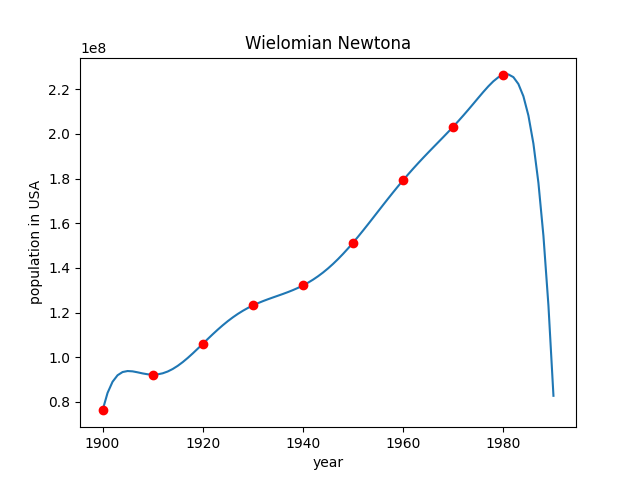
\includegraphics[scale = 0.9]{wykres3.png}
	\end{figure}
	
	Powyższy wykres jest identyczny jak ten stworzony na podstawie macierzy oraz metodą Lagrange'a, co potwierdza poprawność wyznaczonego wielomianu metodą Newtona.
	
	
	
	\subsection*{Zaokrąglone wartości populacji, a wynik interpolacji}
	
	Dane z pierwszej tabeli zaokrąglono do jednego miliona:
	
	\begin{center}
		\begin{tabular}{c|c}
  			\hline 
  			Rok & Zaokraglona populacja\\
  			\hline
  			1900 & 76 000 000 \\
  			1910 & 92 000 000 \\
  			1920 & 106 000 000 \\
  			1930 & 123 000 000 \\
  			1940 & 132 000 000 \\
  			1950 & 151 000 000 \\
  			1960 & 179 000 000 \\
  			1970 & 203 000 000 \\
  			1980 & 227 000 000 \\
		\end{tabular} 
		
	\end{center}
	
	Następnie rozwiązano rownanie (5), przy czym macierzą $Y$ w tym przypadku były dane z powyższej tabeli. Otrzymane wartości współczynnikow (Wsp-Z) porównano w tabeli z wartościami współczynników obliczonych dla niezaokraglonych danych (Wsp-NZ).
	
	
	\begin{center}
		\begin{tabular}{|c|c|c|}
  			\hline 
  			Numer wspolczynnika & Wsp-NZ & Wsp-Z\\
  			\hline
  			1 & $1.32164569 \cdot 10^8$ & $1.32000000 \cdot 10^8$ \\
  			2 & $4.61307656 \cdot 10^7$ & $4.59571429 \cdot 10^7$ \\
  			3 & $1.02716315 \cdot 10^8$ & $1.00141270 \cdot 10^8$ \\
  			4 & $1.82527130 \cdot 10^8$ & $1.81111111 \cdot 10^8$ \\
  			5 & $-3.74614715 \cdot 10^8$ & $-3.56755556 \cdot 10^8$ \\
  			6 & $-3.42668456 \cdot 10^8$ & $-3.38488889 \cdot 10^8$ \\
  			7 & $6.06291250 \cdot 10^8$ & $5.70311111 \cdot 10^8$ \\
  			8 & $1.89175576 \cdot 10^8$ & $1.86920635 \cdot 10^8$ \\
  			9 & $-3.15180235 \cdot 10^8$ & $-2.94196825 \cdot 10^8$ \\
  			\hline
		\end{tabular} 
		
	\end{center}
	
	Na podstawie tych współczynników wyznaczono wielomian interpolujacy zaokrąglone punkty i wykonano jego wykres:
	
	
	\begin{figure}[h]
    		\centering
  		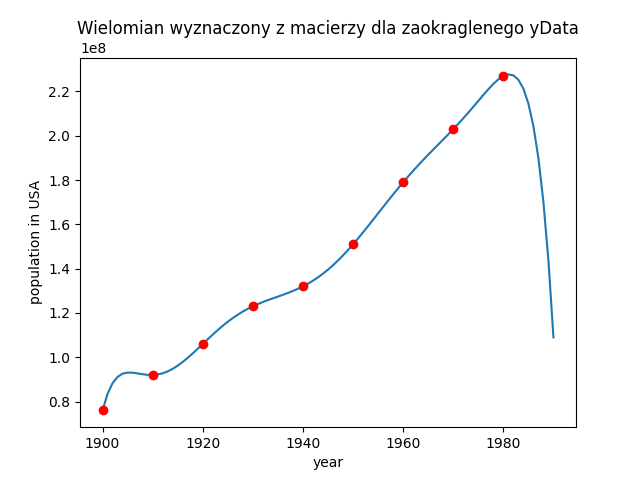
\includegraphics[scale = 0.9]{wykres4.png}
	\end{figure}
	
	Jak można zauważyć, wykres ten jest bardzo podobny do wykresów powstałych na podstawie niezaokrąglonych danych. Ponadto tabela znajdująca się powyżej pokazuje, że wartości otrzymanych współczynników są bardzo zbliżone do wartości odpowiadających im współczynników obliczonych z niezaokrąglonych danych.
	
	
	
	
	
	
	
	
	
	
	
	
	
	
	
	
	
	
	
	
	
	
	
	
\end{document}